\section{Obermarck's algorithm}

Consider the following waiting conditions:
\begin{itemize}
    \item Node $A$: $E_B \rightarrow t_1, t_1 \rightarrow t_2, E_C \rightarrow t_2, t_2 \rightarrow t_3, t_3 \rightarrow E_B, E_B \rightarrow t_4, t_4 \rightarrow t_3$
    \item Node $B$: $E_A \rightarrow t_3, t_3 \rightarrow t_5, t_5 \rightarrow t_6, t_6 \rightarrow E_C, E_C \rightarrow t_7, t_7 \rightarrow t_6, t_9 \rightarrow t_4,t_4 \rightarrow E_A, t_1 \rightarrow E_A$
    \item Node $C$: $E_B \rightarrow t_6, t_6 \rightarrow t_8, t_8 \rightarrow t_2, t_2 \rightarrow E_A, t_7 \rightarrow E_B$
\end{itemize}
Simulate the Obermarck algorithm and indicate whether there is a distributed deadlock.
    
\paragraph*{Solution}
We need to construct the graph with the given constraints, that is: 
\begin{figure}[H]
    \centering
    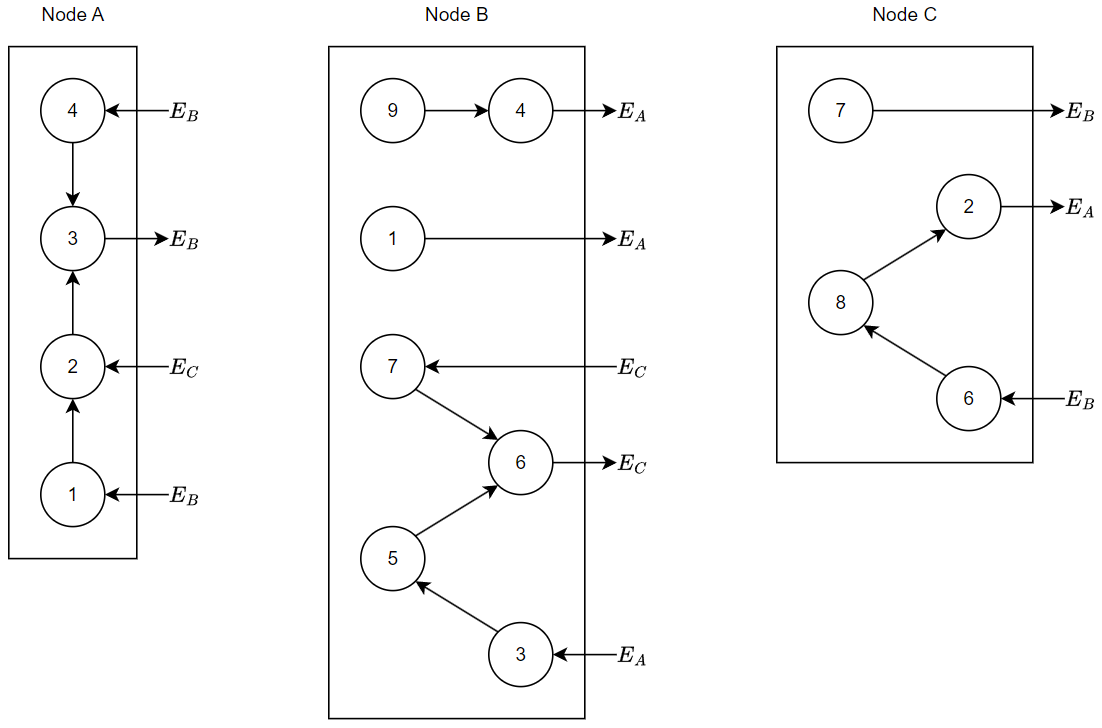
\includegraphics[width=0.6\linewidth]{images/Ob1.png}
\end{figure}
We have to check all the nodes where the sender has a lower value than the receiver. In this case we have that the update is sent to the 
other distributed node. The interesting cases are highlighted in the image. So, we now have to add the nodes: 
\begin{itemize}
    \item $4 \rightarrow 3$ in $E_B$. 
    \item $7 \rightarrow 6$ in $E_C$. 
    \item $6 \rightarrow 2$ in $E_A$. 
\end{itemize}
If the numbered node is not present we can add it to the graph of the distributed node. We obtain the following graphs: 
\begin{figure}[H]
    \centering
    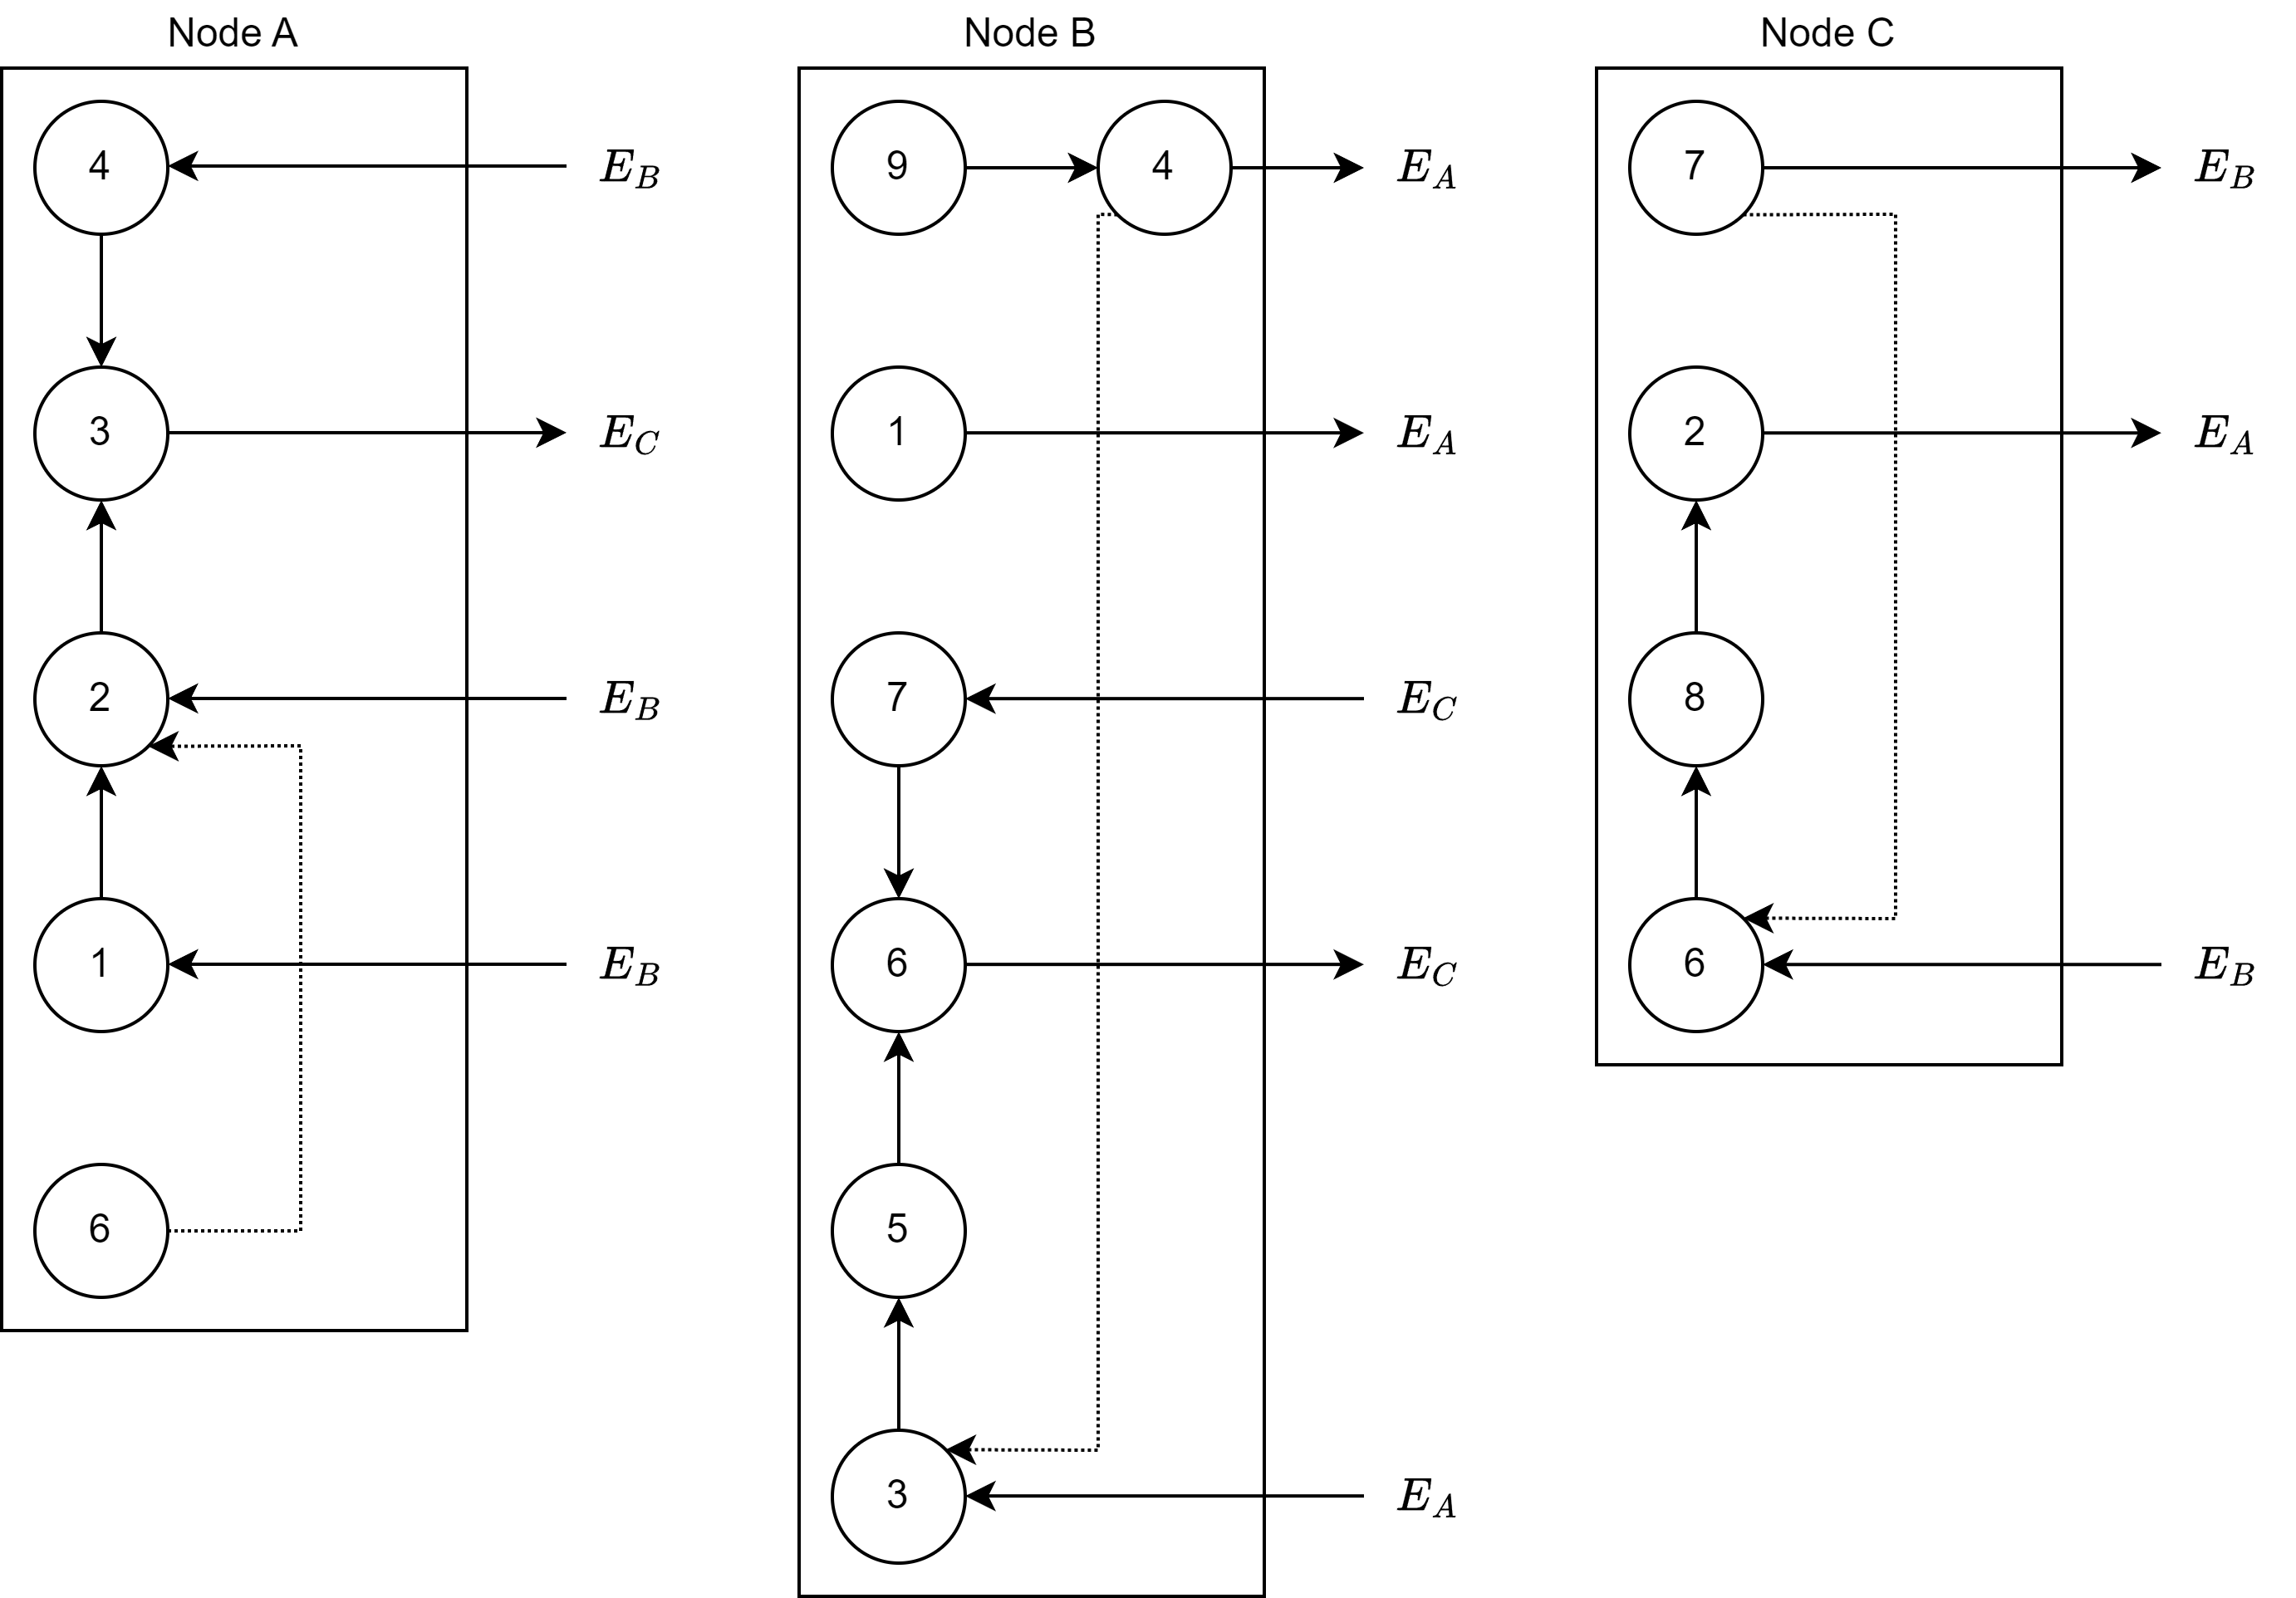
\includegraphics[width=0.6\linewidth]{images/Ob2.png}
\end{figure}
We have to check if other messages are sent. We have:
\begin{itemize}
    \item $6 \rightarrow 3$ in $E_B$. 
\end{itemize}
So the updated graph is: 
\begin{figure}[H]
    \centering
    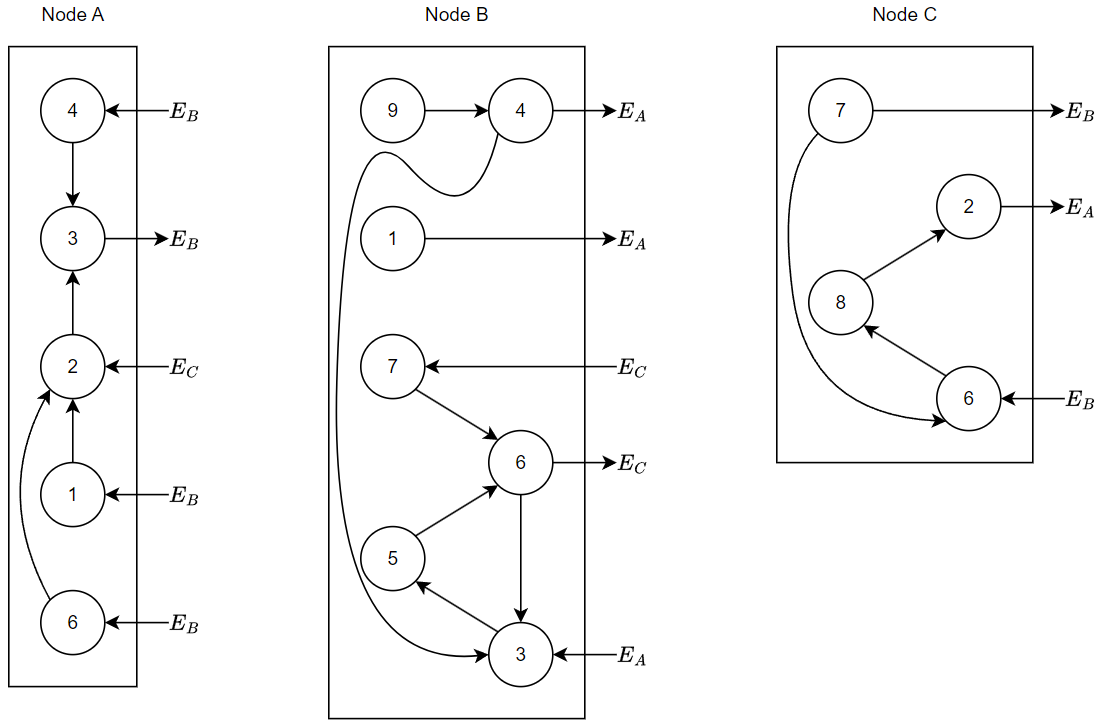
\includegraphics[width=0.6\linewidth]{images/Ob3.png}
\end{figure}
We have found a cycle, so there is a deadlock. 